%
% teil1.tex -- Beispiel-File für das Paper
%
% (c) 2020 Prof Dr Andreas Müller, Hochschule Rapperswil
%
% !TEX root = ../../buch.tex
% !TEX encoding = UTF-8
%
\section{Oberflächenwellen im seichten Gewässer
\label{luke:section:SeichtenGewaesser}}
\kopfrechts{Oberflächenwellen im seichten Gewässer}

In diesem Abschnitt werden wir den Fall betrachten, dass wir eine Oberflächenwelle im seichten Gewässer haben. 
\index{seicht}%
Jedoch variiert die Definition von seichten Gewässer je nach Kontext. 
Im Allgemeinen nennt man Gewässer seicht, wenn diese eine große horizontale Ausdehnung im Vergleich zur Tiefe haben. 
Dabei gibt es keine maximale Tiefe bis zu der ein Gewässer als seicht angenommen wird.
In der Hydrodynamik wird von seichtem bzw. flachem Wasser gesprochen, wenn die Wellenlänge der betrachteten Wasserwelle relativ groß im Vergleich zur Tiefe ist.
\index{Hydrodynamik}%
Im folgendem wird ein Ansatz hergeleitet, welcher aus Vereinfachungen und bekannter Formeln für seichte Gewässer besteht.
Mit dem Ansatz wird eine unbeschränkte Lösung berechnet, welche die Saint-Venant-Gleichungen ergeben.
\index{Saint-Venant-Gleichung}%
Durch Vereinfachung der Saint-Venant-Gleichungen wird die nichtlineare partielle Differenzialgleichung von Burgers hergeleitet, sowie Rückschlüsse auf die Lösung der allgemeinen nichtlinearen eindimensionalen Wellengleichung werden gezogen. 
\index{Burgers}

\subsection{Wahl eines einfachen Ansatzes}
Zuerst definieren wir das Geschwindigkeitsfeld $\bm{u}(\bm{x},z,t)$ bzw. die Ausbreitung der Welle entlang der Horizontalen.
Dabei stößt man in der Literatur auf die Reihenentwicklung
\begin{align}
	\bm{u}(\bm{x},z,t) = \check{\bm{u}}(\bm{x},z,t) - \frac{1}{2} (z + h)^2 \nabla^2 \check{\bm{u}}(\bm{x},z,t) + \frac{1}{24} (z + h)^4 \nabla^4 \check{\bm{u}}(\bm{x},z,t) + \ldots,
\end{align}
welche sich dafür bewährt hat.
Die Entwicklung beschreibt eine lange Welle in seichten Wasser, welche sich entlang eines horizontalen undurchlässigen Bodens bei $z = -h$ ausbreitet.

Um die Berechnungen einfach zu halten wird für die Funktionen $\phi (\bm{x},z,t)$ und $\bm{u} (\bm{x},z,t)$, in Bezug auf die vertikale Richtung $z$, als konstant angenähert, durch die Mittelung über die Wassertiefe \eqref{luke:Mittelung_Wassertiefe}.
Die Funktion $v$ wird auch als lineare Funktion in Bezug auf $z$ angenähert. 
Konkret erhalten wir dadurch den Ansatz
\begin{equation}
\phi(\bm{x},z,t) \approx \bar{\phi}(\bm{x}, t),
\quad
\bm{u}(\bm{x},z,t) \approx \bar{\bm{u}}(\bm{x}, t),
\quad
v(\bm{x},z,t)
\approx
\biggl(\frac{z + h}{\eta(\bm{x}, t) + h}\biggr) \tilde{v}(\bm{x}, t),
\label{luke:Ansatz_Geschw}
\end{equation}
für die Geschwindigkeit.
Dieser Ansatz findet oft in der Modellierung von seichten Gewässern Verwendung, weil dieser gut die Bewegung des Wassers in der Nähe der Oberfläche beschreibt.
Die Lagrange-Multiplikatoren $\mu(\bm{x},z,t)$ und $\upsilon(\bm{x},z,t)$ werden ebenfalls entsprechend dem Ansatz
\begin{equation}
\bm{\mu}(\bm{x},z,t) \approx \bar{\bm{\mu}}(\bm{x}, t),
\quad
\upsilon(\bm{x},z,t)
\approx
\biggl(\frac{z + h}{\eta(\bm{x}, t) + h}\biggr)\tilde{\upsilon}(\bm{x}, t),
\label{luke:Ansatz_Multiplikatoren}
\end{equation}
angenähert.
Die beiden Ansätze \eqref{luke:Ansatz_Geschw} und \eqref{luke:Ansatz_Multiplikatoren} werden in die Lagrange-Funktion \eqref{luke:Luke_Lagrangian_umgeschrieben} eingefügt.
Damit wird die Lagrange-Funktion zu
\begin{align*}
L&=
L(\bm{x},z,t,\eta,\phi,\bm{u}, v, \bm{\mu},\upsilon,\phi_t,\phi_x,\phi_y,\phi_z)
\\
&=
\biggl(\frac{\partial \eta(\bm{x}, t)}{\partial t}
+
\bar{\bm{\mu}}  \nabla \eta(\bm{x}, t)
-
\widetilde{\upsilon}\biggr)\rho \bar{\phi}
-
\frac{1}{2} \rho g \eta(\bm{x}, t)^2
\\
&\quad+
\rho\int_{-h}^{\eta(\bm{x}, t)}
\bigg[ \bar{\bm{\mu}}  \bar{\bm{u}} - \frac{1}{2} \bar{\bm{u}}^2
+
\biggl(\frac{z + h}{\eta(\bm{x}, t) + h}\biggr)
\tilde{\upsilon}
\biggl(\frac{z + h}{\eta(\bm{x}, t) + h}\biggr)\tilde{v}
- \frac{1}{2} \biggl(\frac{z + h}{\eta(\bm{x}, t) + h}\biggr)\tilde{v}^2 
\\
&\quad+\biggl(\nabla \bar{\bm{\mu}}
+ \frac{\partial}{\partial z}
\biggl(\frac{z + h}{\eta(\bm{x}, t) + h}\biggr)\tilde{\upsilon}\biggr)
\bar{\phi} \bigg] dz.
\end{align*}
Das Integral wird umgeformt und für leichteres Verständnis auf drei Teile
\begin{align*}
L&=
\biggl(\frac{\partial \eta(\bm{x}, t)}{\partial t}
+
\bar{\bm{\mu}}  \nabla \eta(\bm{x}, t)
-
\widetilde{\upsilon}\biggr)\rho \bar{\phi}
-
\frac{1}{2}\rho g \eta(\bm{x}, t)^2
\\
&\qquad+
\rho\int_{-h}^{\eta(\bm{x}, t)}
\biggl[
\nabla \bar{\bm{\mu}}\bar{\phi} + \bar{\bm{\mu}}\bar{\bm{u}}
- \frac{1}{2} \bar{\bm{u}}^2
\biggr]\, dz
+
\rho\int_{-h}^{\eta(\bm{x}, t)}
\biggl[
\biggl(\frac{z + h}{\eta(\bm{x}, t) + h}\bigr)^2
\biggl(\tilde{\upsilon}\tilde{v} - \frac{1}{2} \tilde{v}^2\biggr)
\biggr]\, dz
\\
&\qquad+
\rho\int_{-h}^{\eta(\bm{x}, t)}
\biggl[
\biggl(\frac{\partial}{\partial z} \biggl(\frac{z + h}{\eta(\bm{x}, t) + h}\biggr)\tilde{\upsilon} \bar{\phi}
\biggr)
\biggr]\, dz,
\end{align*}
aufgeteilt.
Die drei Integrale werden aufgelöst, wobei
$\left(\frac{\partial}{\partial z}
\left(\frac{z + h}{\eta(\bm{x}, t) + h}\right)
\tilde{\upsilon} \bar{\phi}
\right)
=
\frac{\tilde{\upsilon} \bar{\phi}}{\eta(\bm{x}, t) + h}$
ist.
Das ergibt
\begin{align*}
L&=
\biggl(\frac{\partial \eta(\bm{x}, t)}{\partial t}
+
\bar{\bm{\mu}} \nabla \eta(\bm{x}, t)
-
\widetilde{\upsilon}\biggr)\rho \bar{\phi}
-
\frac{1}{2}\rho g \eta(\bm{x}, t)^2
+
\rho(\eta(\bm{x}, t) + h)
\biggl(\nabla \bar{\bm{\mu}}\bar{\phi} + \bar{\bm{\mu}}\bar{\bm{u}}
- \frac{1}{2} \bar{\bm{u}}^2\biggr)
\\
&\qquad
+
\rho(\eta(\bm{x}, t) + h)
\biggl(\frac{1}{3}\tilde{\upsilon}\tilde{v} - \frac{1}{6}\tilde{v}^2 \biggr)
+
\rho\tilde{\upsilon} \bar{\phi}.
\end{align*}
Somit erhalten wir die einfache Lagrange-Funktion
\begin{align*}
&L(\bm{x},z,t,\eta,\phi,\bm{u}, v, \bm{\mu},\upsilon,\phi_t,\phi_x,\phi_y,\phi_z)
\\
&\qquad
=
\biggl(\frac{\partial \eta(\bm{x}, t)}{\partial t}
+
\bar{\bm{\mu}} \nabla \eta(\bm{x}, t)
\biggr)\rho \bar{\phi}
-
\frac{1}{2}\rho g \eta(\bm{x}, t)^2
\\
&\qquad\qquad
+
\rho(\eta(\bm{x}, t) + h)
\biggl(\nabla \bar{\bm{\mu}}\bar{\phi} + \bar{\bm{\mu}}\bar{\bm{u}} - \frac{1}{2} \bar{\bm{u}}^2 + \frac{1}{3} \tilde{\upsilon}\tilde{v} - \frac{1}{6}\tilde{v}^2\biggr)
\end{align*}
für eine Oberflächenwasserwelle in seichten Gewässer.
Diese Funktion kann mittels des Satzes von Green umgeformt werden.
Diese Umformung wurde von Didier Clamond und Denys Dutykh \cite{luke:CLAMOND201225} durchgeführt.
Dabei ergibt sich die äquivalente Lagrange-Funktion
\begin{align}
&L(\bm{x},z,t,\eta,\phi,\bm{u}, v, \bm{\mu},\upsilon,\phi_t,\phi_x,\phi_y,\phi_z)
\notag
\\
&\qquad=
\rho\bar{\phi}\frac{\partial \eta(\bm{x}, t)}{\partial t}
-
\frac{1}{2} \rho g \eta(\bm{x}, t)^2
+
\rho(\eta(\bm{x}, t) + h)
\biggl(
\bar{\bm{\mu}}\bar{\bm{u}}
-
\frac{1}{2} \bar{\bm{u}}^2 
+
\frac{1}{3} \tilde{\upsilon}\tilde{v}
-
\frac{1}{6}\tilde{v}^2
-
\bar{\bm{\mu}}\nabla \bar{\phi}
\biggr).
\label{luke:Lagrangian_mit_Ansatz}
\end{align}
Im nächsten Schritt werden wir diese Lagrange-Funktion \eqref{luke:Lagrangian_mit_Ansatz} nehmen und das Variationsprinzip anwenden.

\subsection{Berechnung der unbeschränkten Lösung}
Ohne weitere Einschränkungen werden wir nun die Minimierung über
das Variationsprinzip durchführen und die Euler-Lagrange-Gleichungen
aufstellen.
Dazu werden partiellen Ableitungen berechnet:
\begin{align}
\frac{\partial L}{\partial \bar{\bm{u}}} &= 0
,\quad
\frac{\partial L}{\partial \bar{\bm{\mu}}} = 0
,\quad
\frac{\partial L}{\partial \tilde{v}} = 0
,\quad
\frac{\partial L}{\partial \tilde{\upsilon}} = 0
,\quad
\frac{\partial L}{\partial \bar{\phi}} = 0
,\quad
\frac{\partial L}{\partial \eta} = 0
\notag
\\
\frac{\partial L}{\partial \bar{\bm{u}}}
&=
\frac{\partial \mathscr{}}{\partial \bar{\bm{u}}}
\biggl(\bar{\bm{\mu}}\bar{\bm{u}} - \frac{1}{2} \bar{\bm{u}}^2\biggr)
= 0
\nonumber \\ 
\frac{\partial L}{\partial \bar{\bm{u}}}
&=
\bar{\bm{\mu}} - \bar{\bm{u}}
= 0
\label{luke:Variation_nach_u} 
\\
%Variation nach mu
\frac{\partial L}{\partial \bar{\bm{\mu}}}
&=
\frac{\partial L}{\partial \bar{\bm{\mu}}}
( \bar{\bm{\mu}}\bar{\bm{u}}-\bar{\bm{\mu}}\nabla \bar{\phi} )
= 0
\nonumber \\
\frac{\partial L}{\partial \bar{\bm{\mu}}}
&=
\bar{\bm{u}}-\nabla \bar{\phi}
= 0
\label{luke:Variation_nach_mu}
\\
%Variation nach v
\frac{\partial L}{\partial \tilde{v}}
&=
\frac{\partial \mathscr{}}{\partial \tilde{v}}
\biggl(\frac{1}{3} \tilde{\upsilon}\tilde{v} - \frac{1}{6} \tilde{v}^2\biggr)
= 0
\nonumber \\
\frac{\partial L}{\partial \tilde{v}}
&=
\tilde{\upsilon}-\tilde{v}
= 0
\label{luke:Variation_nach_v}
\\
%Variation nach upsilon
\frac{\partial L}{\partial \tilde{\upsilon}}
&=
\frac{\partial \mathscr{}}{\partial \tilde{\upsilon}}
\biggl(\frac{1}{3} \tilde{\upsilon}\tilde{v}\biggr)
= 0
\nonumber \\	
\frac{\partial L}{\partial \tilde{\upsilon}}
&=
\tilde{v}
= 0
\label{luke:Variation_nach_upsilon}
\\
%Variation nach phi
\frac{\partial L}{\partial \bar{\phi}}
&=
\frac{\partial \mathscr{}}{\partial \bar{\phi}}
\biggl(
\rho\bar{\phi}\frac{\partial \eta(\bm{x}, t)}{\partial t}
-
\rho(\eta(\bm{x}, t) + h)\bar{\bm{\mu}}\nabla \bar{\phi}
\biggr)
= 0
\nonumber \\
\frac{\partial L}{\partial \bar{\phi}}
&=
\frac{\partial \eta(\bm{x}, t)}{\partial t} -
\nabla\bigl((\eta(\bm{x}, t)+ h)\bm{\bar{\mu}}\bigr)
= 0
\label{luke:Variation_nach_phi}
\\
%Variation nach eta
\frac{\partial L}{\partial \eta}
&=
\frac{\partial \mathscr{}}{\partial \eta}
\bigg(\rho\bar{\phi}\frac{\partial \eta(\bm{x}, t)}{\partial t}
-
\frac{1}{2} \rho g \eta(\bm{x}, t)^2
+
\nonumber \\
&\qquad\quad
\rho(\eta(\bm{x}, t) + h)
\biggl(
\bar{\bm{\mu}}\bar{\bm{u}}
-
\frac{1}{2} \bar{\bm{u}}^2 
+
\frac{1}{3} \tilde{\upsilon}\tilde{v}
-
\frac{1}{6}\tilde{v}^2
-
\bar{\bm{\mu}}\nabla \bar{\phi}
\biggr)
\bigg)
= 0
\nonumber \\
\frac{\partial L}{\partial \eta}
&=
-
\frac{\partial \bar{\phi}}{\partial t}
-
g\eta(\bm{x}, t)
+
\bar{\bm{\mu}}\bar{\bm{u}}
-
\frac{1}{2} \bar{\bm{u}}^2 
+
\frac{1}{3} \tilde{\upsilon}\tilde{v}
-
\frac{1}{6}\tilde{v}^2
-
\bar{\bm{\mu}}\nabla \bar{\phi}
= 0.
\label{luke:Variation_nach_eta}
\end{align}

Wie zu erwarten war, ergibt die Gleichung \eqref{luke:Variation_nach_u}
und \eqref{luke:Variation_nach_v}, dass $\bar{\bm{\mu}} = \bar{\bm{u}}$
und $\tilde{\upsilon} = \tilde{v}$ ist.
Dieser Zusammenhang wurde bereits beim Variieren der Lagrange-Funktion \eqref{luke:Luke_Lagrangian_mit_Multi} gezeigt.
Die Gleichung \eqref{luke:Variation_nach_mu} und \eqref{luke:Variation_nach_upsilon} zeigen, dass die Geschwindigkeitsfelder genau einem Geschwindigkeitspotential entsprechen und das die vertikale Geschwindigkeit konstant bleibt. 
Für uns interessant sind die Gleichungen \eqref{luke:Variation_nach_phi} und \eqref{luke:Variation_nach_eta}.
Diese lassen sich nämlich umschreiben zu 
\begin{align}
	\frac{\partial H}{\partial t} + \nabla \cdot [H \bar{\bm{u}}] &= 0
	\label{luke:Variation_loesung_1}
\\
	\frac{\partial \bar{\bm{u}}}{\partial t} + (\bar{\bm{u}} \cdot \nabla) \bar{\bm{u}} + g \nabla H &= 0,
	\label{luke:Variation_loesung_2}
\end{align}
wobei $H = \eta(\bm{x},t) + h$ die Gesamtwassertiefe ist.

Gleichung \eqref{luke:Variation_loesung_1} und
\eqref{luke:Variation_loesung_2} ergeben die Saint-Venant-Gleichungen,
wobei die Gleichung \eqref{luke:Variation_loesung_1} die
Kontinuitätsgleichung ist.
\index{Kontinuitätsgleichung}%
Diese finden Verwendung bei der Modellierung von langen Wellen in unbeschränkten seichten Gewässern.
\index{lange Wellen}%
Bei diesen Gleichungen handelt es sich um nichtlineare Differenzialgleichungen, welche über verschiedene numerischen Methoden gelöst werden können.
Da es in dieser Arbeit nicht um das numerische lösen von Differenzialgleichungen handelt, sondern um die Demonstrierung der Anwendung und Vorteile des Variationsprinzip, wird im nächsten Kapitel die Gleichung \eqref{luke:Variation_loesung_2} genauer betrachtet.
Durch Vereinfachung der Gleichung wird die nicht viskose Burgers-Gleichung
erlangt und Ähnlichkeiten zur Lösung der linearen Wellengleichung
im eindimensionalen Fall werden dargestellt.
\index{Burgers-Gleichung}%

\subsection{Interpretation und Anwendung der unbeschränkten Lösung}
Wenn für die Gleichung \eqref{luke:Variation_loesung_2} angenommen wird, dass über die gesamte Zeit $t$ keine Änderung der Gesamtwassertiefe $ \nabla H = 0 $ erfolgt und die horizontale Koordinate $y$ konstant $\frac{\partial \bar{\bm{u}}}{\partial y} = 0$ ist, ergibt sich daraus die Burgers-Gleichung
\begin{equation}
	\frac{\partial \bar{u}}{\partial t} + \bar{u} \frac{\partial \bar{u}}{\partial x} = 0
	\label{luke:Burgers_DG}
\end{equation}
für ein nicht-viskoses Fluid.
Bei der Burgers-Gleichung handelt es sich um eine nichtlineare, homogene und partielle Differentialgleichung.
Die Differentialgleichung wird in der Regel über die Charakteristikenmethode gelöst. 
\index{Charakteristikenmethode}%
Dabei entsteht die Lösung
\[
\bar{u}(x,t) = f(\xi) = f(x-\bar{u}t),\quad \xi = x-f(\xi)t,
\]
wobei $\xi$ der Punkt auf der $x$-Achse ist bei $t = 0$ von dort aus die charakteristischen Kurve aus startet.
Diese Lösung beschreibt eine nichtlineare Wellenbewegung in welcher sich die Anfangsform der Welle im Laufe der Zeit ändert.
Sozusagen stellt dies eine Stoßwelle in $x$-Richtung dar.
Damit lässt sich Verhaltensweisen wie Stoßwellenbildung, Singularitäten und Schockwellen beschreiben.
\begin{figure}
	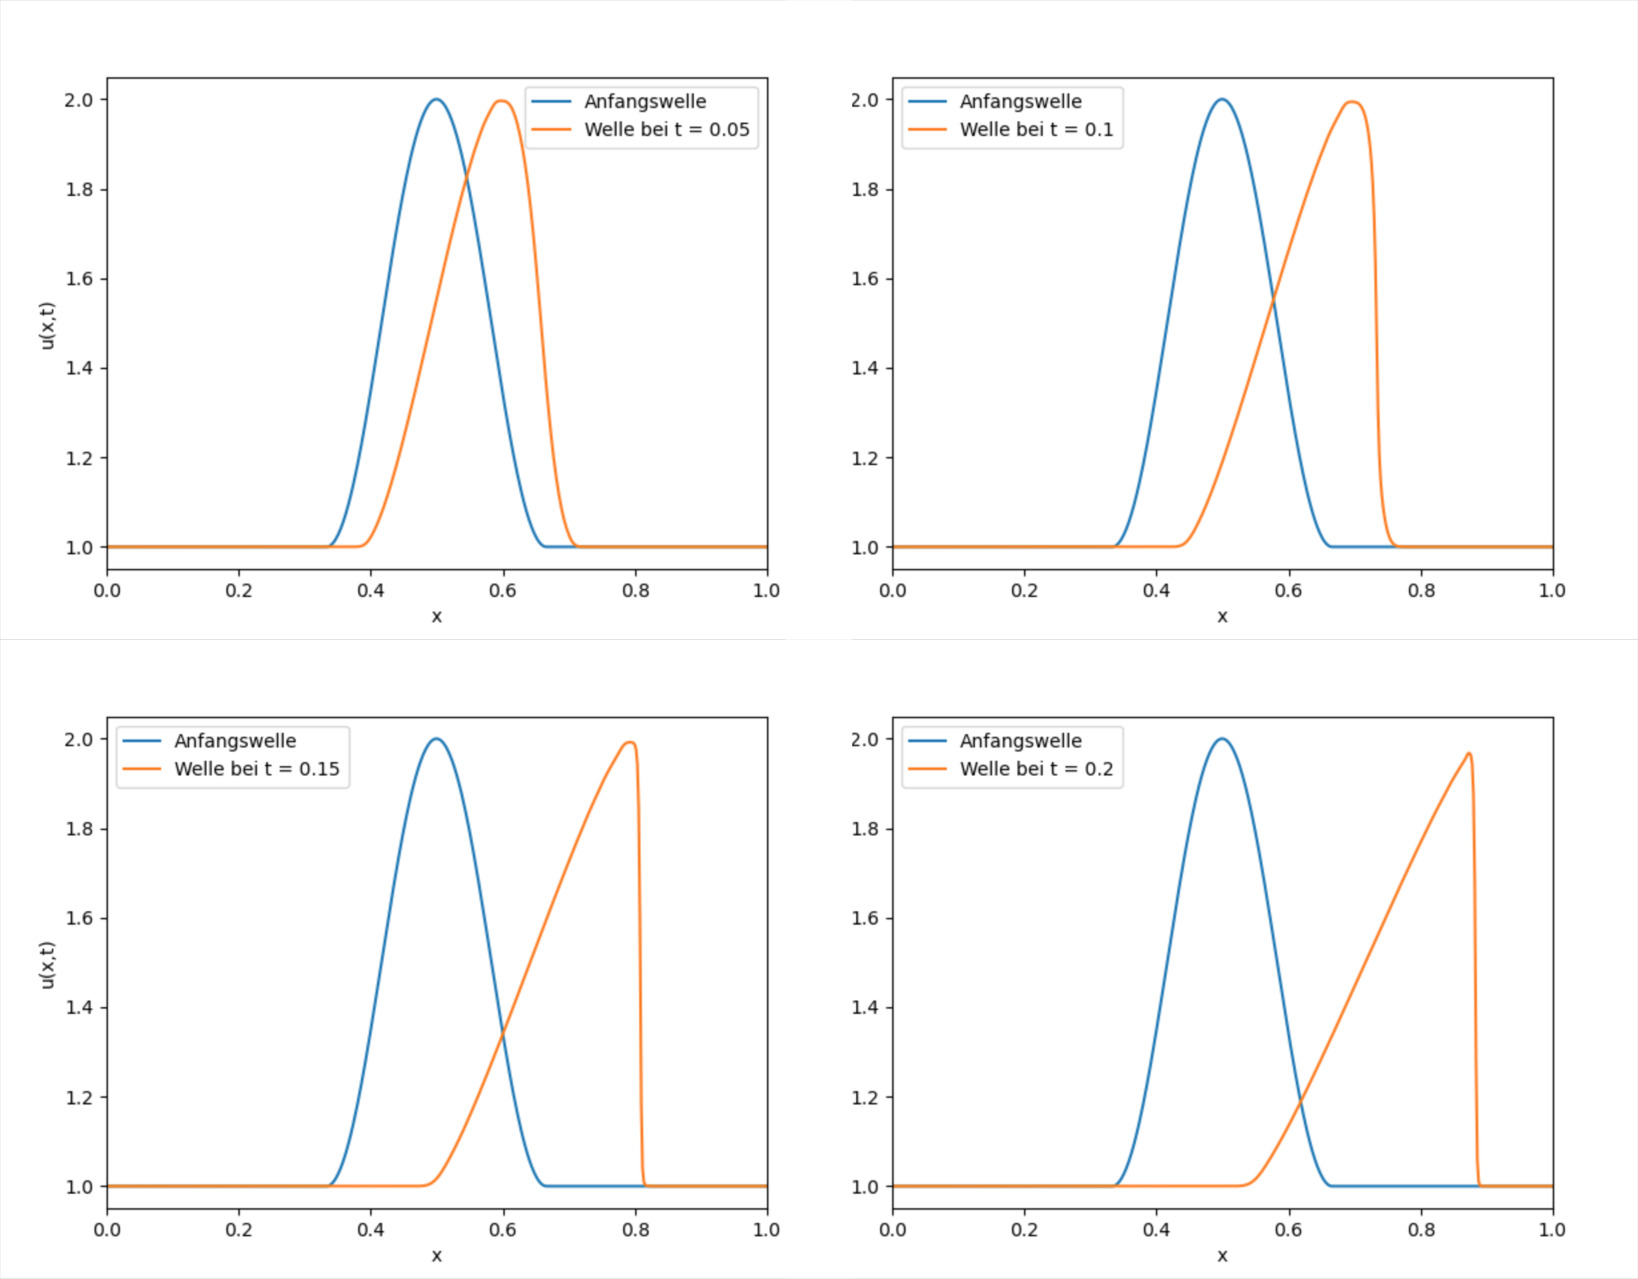
\includegraphics[width=\textwidth]{papers/luke/fig/Burger_Loesung_Welle.jpg}
	\caption{Lösung der Burgers Differenzialgleichung \eqref{luke:Burgers_DG} mit einem $sin(x)^2$ als Welle
		\label{luke:fig:Loesung_Burgers}}
\end{figure}
Abbildung \ref{luke:fig:Loesung_Burgers} zeigt die Lösung der Burgers-Gleichung mit einer nach rechts laufenden Welle, welche zu einem Überschlag der Welle führt.

Die allgemeine lineare Wellengleichung in einer Dimension lautet
\index{lineare Wellengleichung}%
\index{Wellengleichung, linear}%
\[
\partial_t^2 u - a^2 \partial_x^2 u  = 0.
\]
Dabei ist $a$ die Geschwindigkeit der Welle entlang der $x$-Achse.
Diese Wellengleichung kann in einem Bereich von $\Omega = \{(x,t)\mid t >0\}$ mit den Anfangswerten
\[
u(x,0) = u_0(x),\quad \frac{\partial u}{\partial t} = v_0(x),\quad x \in \mathbb{R},
\]
berechnet werden.
Wenn angenommen wird, dass die Geschwindigkeit $a$ konstant ist, kann die Gleichung auf die Differenzialgleichung erster Ordnung
\[
(\partial_t\mp a\partial_x)(\partial_t\pm a\partial_x) u  = 0
\]
 umgeschrieben werden.
Somit ist die Lösung der Gleichung
\begin{equation}
	\partial_t u \mp a\partial_x u = 0,
	\label{luke:Loesung_Wellengleichung}
\end{equation}
erster Ordnung automatisch eine Lösung der Wellengleichung.
Wenn nun die Gleichung \eqref{luke:Variation_loesung_2} hergenommen wird, welche über das Variationsprinzip berechnet wurde, und erneut angenommen wird, dass sich über die gesamte Zeit $t$ keine Änderung der Gesamtwassertiefe $ \nabla H = 0 $ ergibt, sowie die horizontale Koordinate $y$ konstant ist, und diese mit der Lösung der Wellengleichung \eqref{luke:Loesung_Wellengleichung} verglichen wird, dann ist zu erkennen, dass sich die Lösung über die Variation von der Lösung der Wellengleichung unterscheidet anhand dessen wie die Geschwindigkeit der Welle eingebunden ist.
Bei der Betrachtung der beiden Gleichungen
\begin{align}
	\text{Variation: }\frac{\partial \bar{u}}{\partial t} + \bar{u} \frac{\partial \bar{u}}{\partial x} = 0,
	\qquad
	\text{Wellengleichung: }\frac{\partial u}{\partial t} + a \frac{\partial u}{\partial x} = 0,
	\nonumber
\end{align}
lässt es sich leicht erkennen, dass bei der Wellengleichung die Wellengeschwindigkeit $a$ eine Konstante ist, wobei es bei der Lösung der Variation die Wellengeschwindigkeit $\bar{u}$ von der Position $x$ sowie der Zeit $t$ abhängig ist.

